\documentclass[11pt,a4paper]{article}

% Required packages
\usepackage[utf8]{inputenc}
\usepackage[T1]{fontenc}
\usepackage{times} % Times New Roman font
\usepackage{CJK} % For Japanese text support
\usepackage{geometry}
\usepackage{multicol}
\usepackage{setspace}
\usepackage{graphicx}
\usepackage{xcolor}
\usepackage{fancyhdr}
\usepackage{titlesec}
\usepackage{caption}     % For \captionof

% Page geometry setup
\geometry{
    a4paper,
    top=25mm,
    bottom=30mm,
    left=18mm,
    right=18mm
}

% Remove page numbers
\pagestyle{empty}

% Configure two-column layout
% Column width: 83.5mm each, spacing: 7mm
\setlength{\columnsep}{7mm}
\setlength{\columnwidth}{83.5mm}

% Configure section titles (chapter titles)
\titleformat{\section}
{\normalfont\fontsize{11}{13}\bfseries}{\thesection}{1em}{}

\titleformat{\subsection}
{\normalfont\fontsize{11}{13}\bfseries}{\thesubsection}{1em}{}

% Line spacing to achieve approximately 60 lines per column
\linespread{1.0}

% Remove paragraph indentation and add spacing
\setlength{\parindent}{0pt}
\setlength{\parskip}{0.5ex}

\begin{document}

% First page header setup (6 lines from top)
\begin{center}
% Line 1: blank
~\\
% Line 2: Title in English (Times New Roman, 12pt, Center)
{\fontsize{12}{14}\selectfont \textbf{A Multifaceted Exploration of Spatial Openness in Rental Housing: Big Data Analysis Across Tokyo's 23 Wards}}\\
% Line 3: Title in Japanese (MS Mincho, 11pt, Center)
\begin{CJK}{UTF8}{min}
{\fontsize{11}{13}\selectfont 賃貸住宅における空間開放性の多面的探究:東京23区のビッグデータ分析}
\end{CJK}\\
% Line 4: blank
~\\
\end{center}

% Line 5: Affiliation, Student ID, Name (Times New Roman, 11pt, Right-justified)
\begin{flushright}
{\fontsize{11}{13}\selectfont Oki Lab , Student ID: 23M5833, Yuan Liu}
\end{flushright}

% Line 6: blank
~\\

% Main body starts from line 7
\begin{multicols}{2}
\fontsize{11}{13}\selectfont

\section{Introduction}

Spatial openness represents one of the most critical factors influencing customer decision-making in
property selection and serves as a fundamental consideration for designers creating effective
residential spaces. This concept encompasses the perceived spaciousness, visual connectivity, and
flow within living environments, directly impacting occupant satisfaction and quality of life.
Understanding and quantifying spatial openness is therefore essential for both real estate
professionals and architectural designers seeking to optimize residential design.

Traditional approaches to analyzing spatial openness have predominantly relied on structured data
analysis, constrained by the availability and format of existing data sources. These conventional
methods typically depend on standardized metrics such as floor area, room count, and basic
dimensional measurements, which fail to capture the nuanced spatial qualities that truly define
openness. Few studies have successfully leveraged rich, unstructured data sources such as interior
design imagery and madori (floor plan) data to transform these abstract visual elements into
quantifiable statistics that can yield innovative insights.

This research addresses these limitations by proposing a novel methodology that harnesses various
innovative information sources through advanced computational techniques. Our approach integrates
interior images combined with semantic segmentation, floor plan (madori) images processed through
semantic segmentation, and optical image-based visibility graph analysis (VGA). This methodology
breaks the traditional constraints of VGA studies, which have historically depended heavily on data
inputs that require human intervention, such as AutoCAD vectorized maps and proprietary software
like DepthMapX.

Our method incorporates several technical improvements utilizing purely open-source coding
frameworks that significantly accelerate data processing capabilities. These advancements enable
the extension of such analysis to substantially larger datasets, making it possible to extract
meaningful insights from big data when working with unstructured, abstract image datasets. By
largely reducing the need for manual processes typically required by traditional spatial analysis
tools, our approach enables fully automated processing pipelines that can handle large-scale
datasets without human intervention, opening new possibilities for comprehensive urban-scale
studies of residential spatial quality.

\section{Data Source and Preprocessing}

The data source for this study is the rental category of data from the Lifull dataset. In this study, 
we focus on the rental property in Tokyo area, constructed date from 1960 to most recent years. Every 
decades we sampled roughly 1000 to 1500 properties to make the distribution more balanced. Since we 
need clear interior images for interior semseg analysis, clear madori images to extract the VGA distributions,
and compare the properties visual elements from those images to their tabular specs data, we have to screen 
outs those poor quality images and very incomplete infos, after the filtering we have around 6000 
properties left. As illustrated in Figure \ref{fig:samplesize_decades}, our dataset demonstrates a comprehensive coverage 
across Tokyo's 23 wards spanning multiple construction decades. 
% Image inside multicols environment to fit within one column
% \begin{figure}[htbp]
\begin{center}
    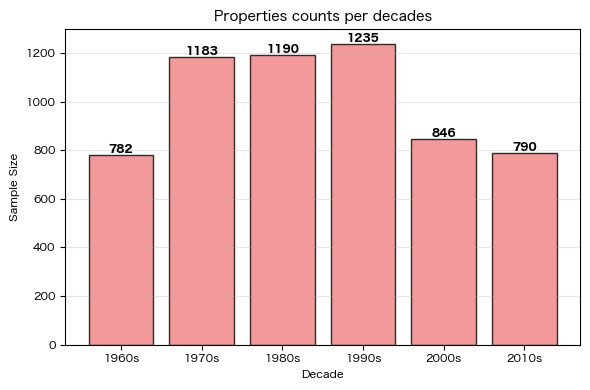
\includegraphics[width=\columnwidth]{plots/samplesize_decades.png}
    \captionof{figure}{Dataset overview showing property construction date distribution across Tokyo's 23 wards.}
    \label{fig:samplesize_decades}
\end{center}
% \end{figure}

The entire data processing pipeline remains stable and fast in this level, the whole 
processing time can be finished within a couple of hours, though depends on the actual specs of the 
machine. We will mention about the details in the thesis when it comes to the actual technical steps.



\section{Quantifying the Openness of Residential Spaces}

We focus on several key quantifiable statistics that might be related to the openness of properties, beyond the 
already existing tabular features such as room types and room area.

From interior data, we first filtered the main living room images, then applied semantic segmentation using the 
Mask2Former model which is pretrained on the ADE20K dataset to ensure that key components such as walls, ceilings, 
and windows can be correctly tagged. We then extract the ratio of their appearance in each image as features for 
later analysis, as shown in Figure \ref{fig:interior_semseg}. 
\begin{flushleft}
    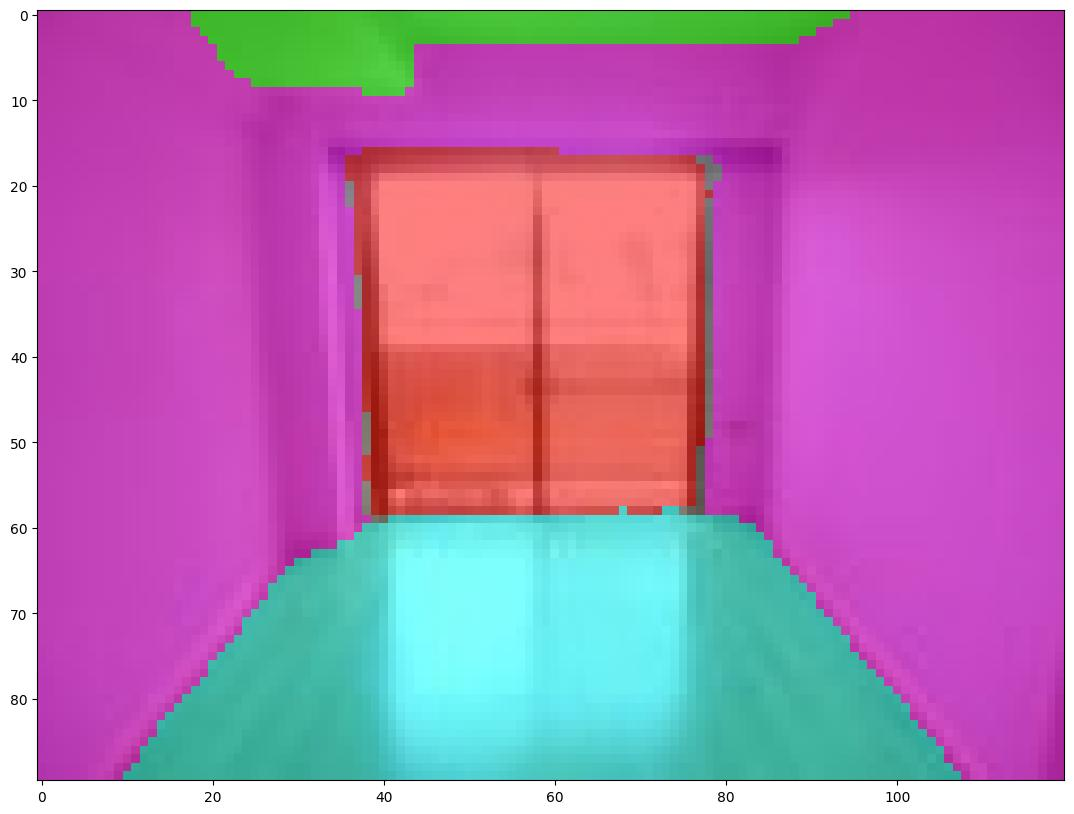
\includegraphics[width=0.8\columnwidth]{plots/exp_lv_semseg_2.jpg}
    \\[0.5em]
    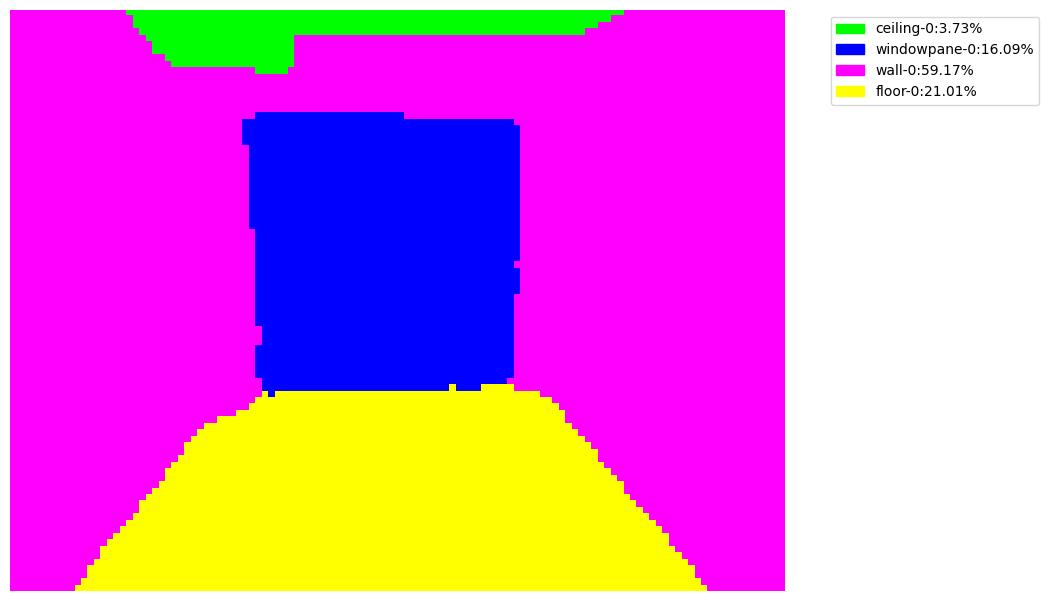
\includegraphics[width=\columnwidth]{plots/exp_lv_semseg_1.jpg}
    \captionof{figure}{Example of interior semantic segmentation results.}
    \label{fig:interior_semseg}
\end{flushleft}


From madori (floorplan) data, we first performed semantic segmentation using a model pretrained on non-floorplan 
data, then utilized a labeled dataset to perform fine-tuning to ensure it can classify floorplan components like 
walls, bedrooms, living rooms, etc. 
\begin{flushleft}
    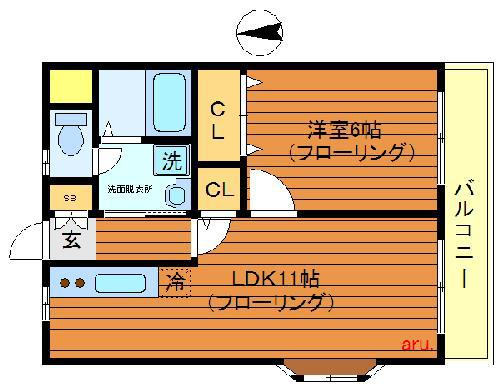
\includegraphics[width=0.7\columnwidth]{plots/exp_maodri_semseg_raw.jpg}
    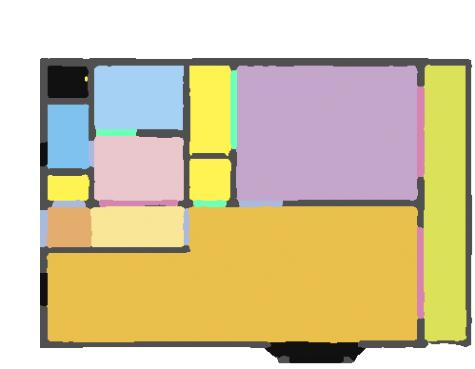
\includegraphics[width=0.7\columnwidth]{plots/exp_madori_semseg_decoded.jpg}
    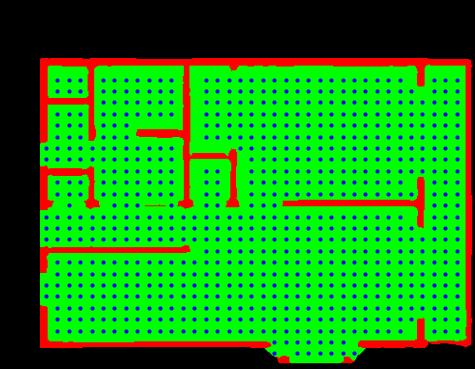
\includegraphics[width=0.7\columnwidth]{plots/exp_madori_semseg_grid.jpg}
    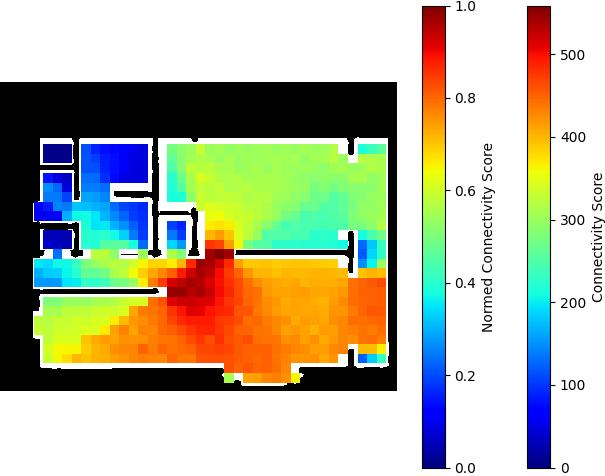
\includegraphics[width=0.7\columnwidth]{plots/exp_madori_semseg_vga.jpg}
    \captionof{figure}{From top to bottom: raw floorplan, the semantic segmentation output, the physical gridding, and the heatmap of VGA.}
    \label{fig:madori_processing}
\end{flushleft}

To obtain VGA scores, we extract the open area by filtering out the background 
and walls. Then, by a given granularity, we create a grid over the area. Since every property has different 
physical dimensions, we normalize the density of gridding by physical size, with each grid cell ranging around 20~cm.

We define the VGA value at each grid node by the number of visible nodes from that node:
\begin{equation}
\label{eq:vga_definition}
S(i) = \sum_{j=1}^{N} V_{ij}
\end{equation}
where $S(i)$ is the visibility score at node $i$, $N$ is the total number of nodes, and $V_{ij} = 1$ if node $j$ 
is visible from node $i$, otherwise $V_{ij} = 0$.
By this method, a VGA heatmap can be generated, and we extract VGA scores by taking the mean, standard deviation, 
minimum/maximum, etc., over the whole property or only living rooms to represent its VGA features. 
The output result with the raw floorplan input for the above processings are demonstrated in the following graph 
as shown in Figure \ref{fig:madori_processing}.

% \fontsize{11}{13}\selectfont
\section{Correlation Analysis Between Subjective Impressions and Openness}

To validate our approach, we analyzed correlations between computed spatial metrics and subjective impressions 
using a pre-trained model by Shimomura et al. that outputs impression scores (q3) from interior images.
We analyzed correlations between q3 impression scores and our extracted observables from both interior images 
and floorplan analysis. Since the model generate the q3 model was trained on the data that only reveal living room
images to users, to reduce the bias, we only extract the vga stats from the floorplan overlayyed with living room
masks. However, no significant correlation is found between them, as shown in Figure \ref{fig:corr_vga_q3}.
The lack of significant correlation stems from a fundamental data source mismatch: the q3 model uses limited-view interior photographs while our VGA analysis processes complete floorplan layouts, capturing different aspects of spatial openness.

We also examined correlations between interior semantic segmentation component ratios and q3 scores. 
After filtering outliers using centered clustering with a 75th percentile cutoff, the results are shown 
in Figures \ref{fig:inter_q3_cluster} and \ref{fig:corr_inter_q3}.

The interior semantic segmentation analysis reveals that window pane and wall components show very weak 
correlation with impression scores, while floor exhibits mild negative correlation and ceiling shows 
moderate negative correlation with q3 scores. This could suggests that shooting angles capturing excessive 
floor area or ceiling visibility negatively impact user evaluations of living room quality 
from single images, emphasizing the importance of balanced camera perspective in interior photography.

\begin{flushleft}
    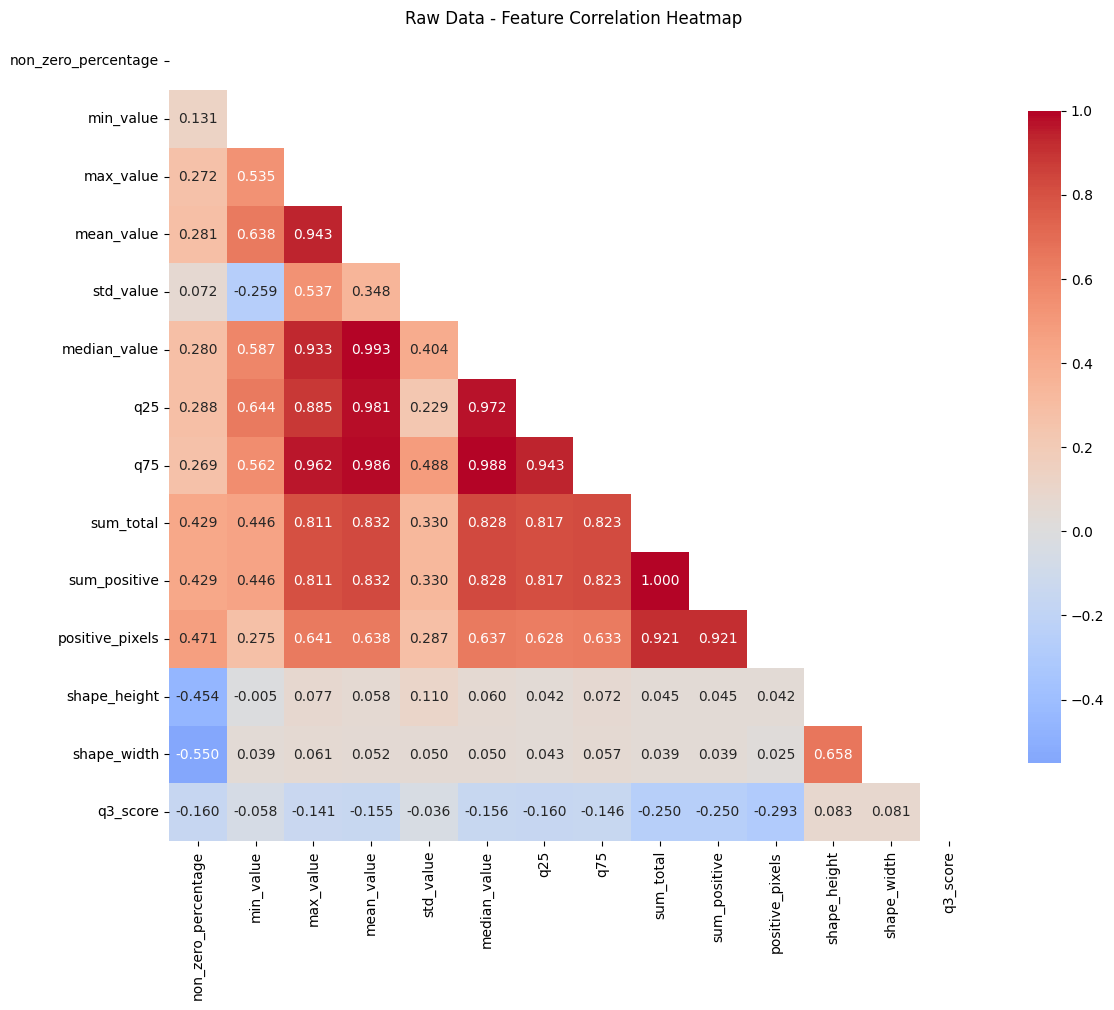
\includegraphics[width=0.9\columnwidth]{plots/corr_vga_q3.png}
    \captionof{figure}{Correlation matrix between q3 impression scores, VGA metrics (mean, std, min, max)}
    \label{fig:corr_vga_q3}
\end{flushleft}

\begin{flushleft}
    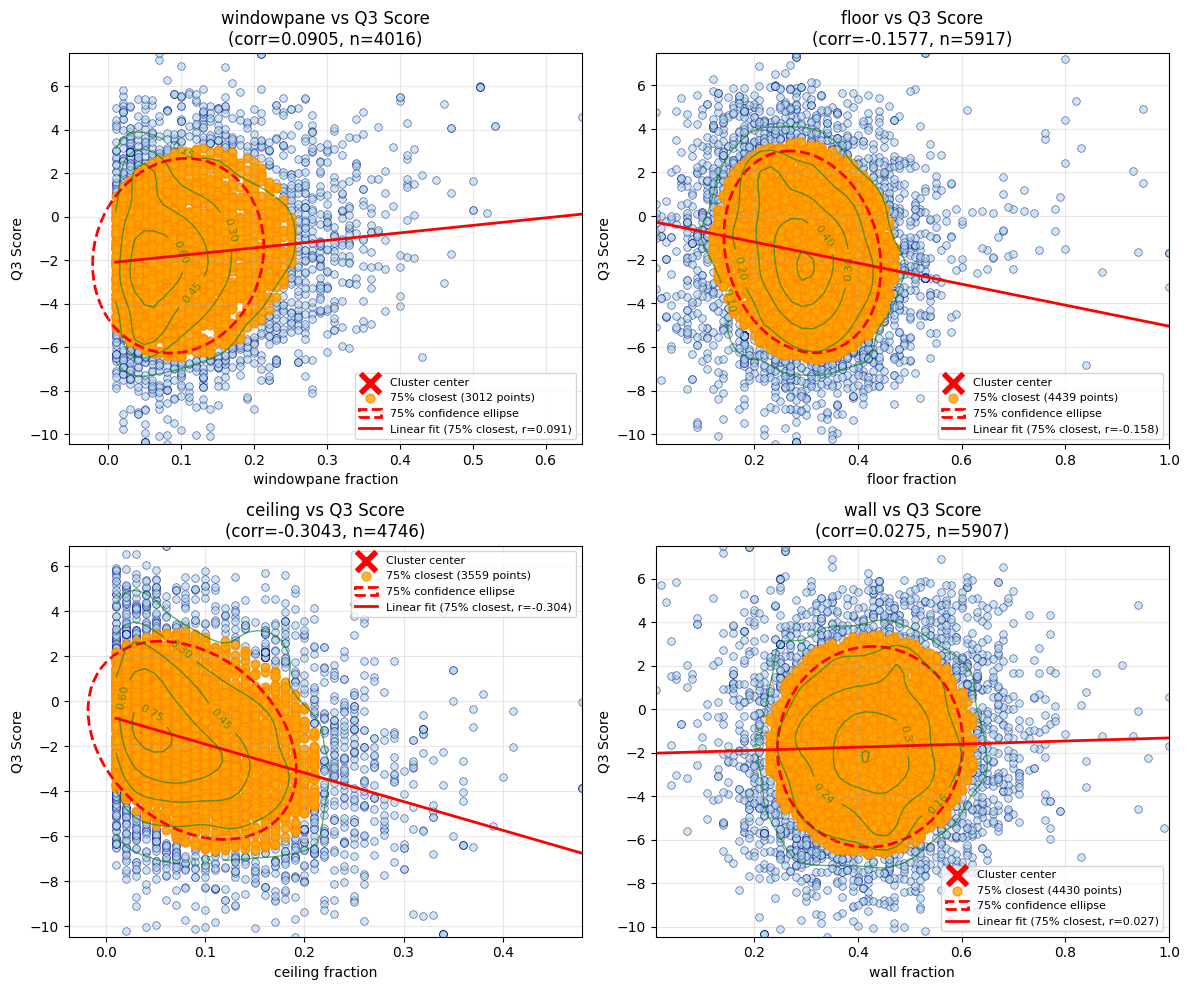
\includegraphics[width=0.9\columnwidth]{plots/inter_q3_cluster.png}
    \captionof{figure}{2D distributions of q3 scores vs. interior semantic segmentation component ratios}
    \label{fig:inter_q3_cluster}
\end{flushleft}

\begin{flushleft}
    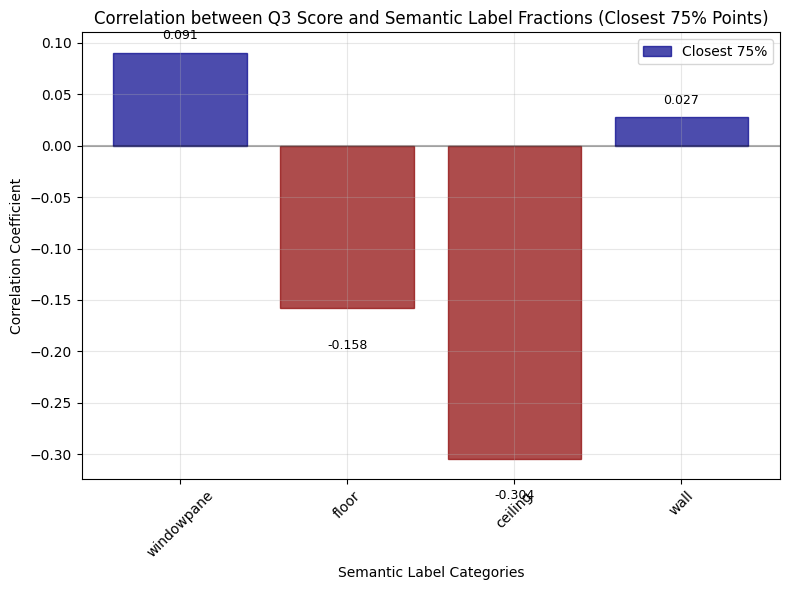
\includegraphics[width=0.9\columnwidth]{plots/corr_inter_q3.png}
    \captionof{figure}{Correlation analysis between q3 scores and semantic segmentation ratios after outlier filtering}
    \label{fig:corr_inter_q3}
\end{flushleft}



We also analyzed correlations between VGA statistics, interior segmentation results, and property data.
Figure \ref{fig:q3_10years_box} shows q3 impression scores by construction decade, revealing trends in 
perceived spatial quality over time. This demonstrates how our framework can identify temporal patterns 
in housing design preferences.

% Additionally, Figure \ref{fig:pie_type} shows the distribution of property types in our dataset, 
% providing context for the composition of analyzed rental properties.

% \begin{flushleft}
%     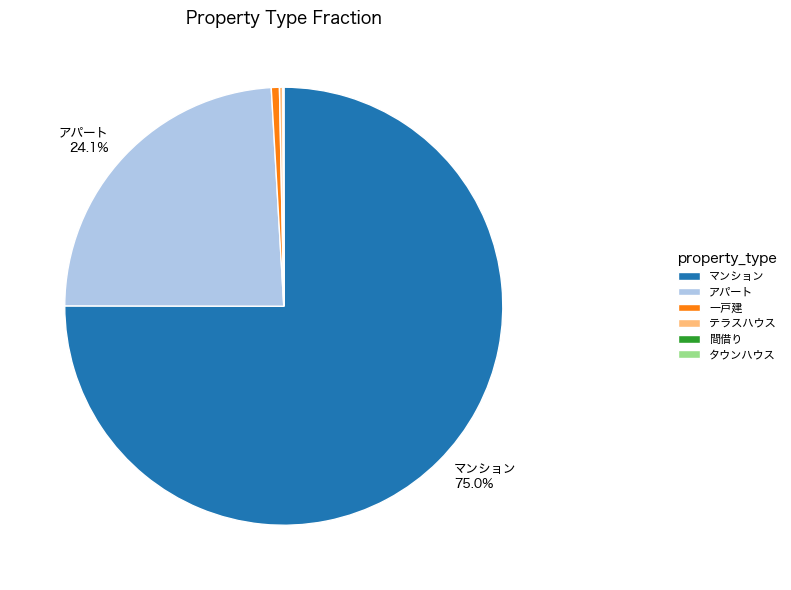
\includegraphics[width=0.7\columnwidth]{plots/pie_type.png}
%     \captionof{figure}{Distribution of property types in the analyzed dataset}
%     \label{fig:pie_type}
% \end{flushleft}


Figure \ref{fig:tokyo23_exp} presents VGA analysis results and q3 impression score distributions across Tokyo's 23 special wards, showing 
spatial distribution patterns of visibility graph metrics and subjective quality assessments. The visualization demonstrates regional 
variations in spatial openness characteristics, providing insights into urban housing design patterns 
at the metropolitan scale.

Detailed analysis will be presented in the full thesis.

\begin{flushleft}
    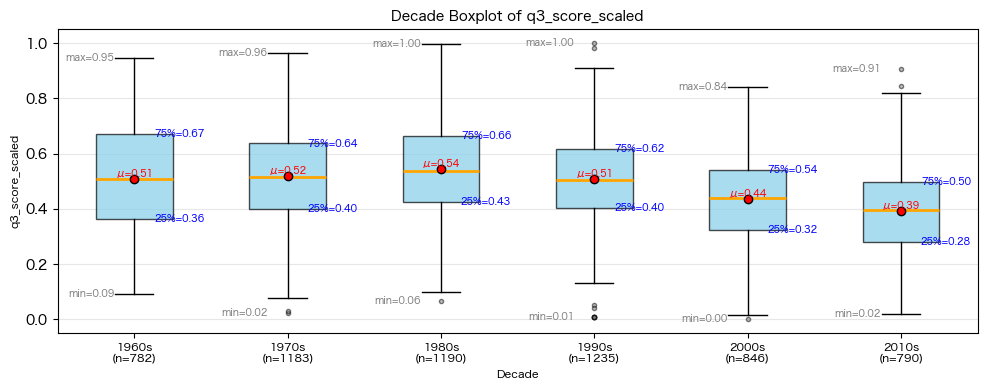
\includegraphics[width=0.9\columnwidth]{plots/q3_10years_box.png}
    \captionof{figure}{Distribution of q3 impression scores by property construction decade}
    \label{fig:q3_10years_box}
\end{flushleft}

\begin{flushleft}
    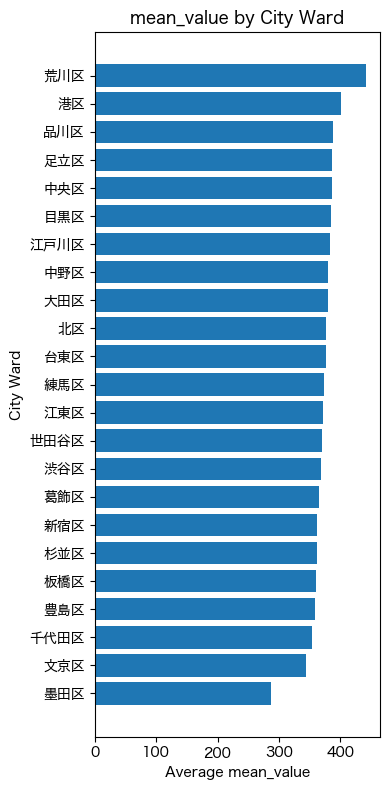
\includegraphics[width=0.45\columnwidth]{plots/tokyo23_vga.png}
    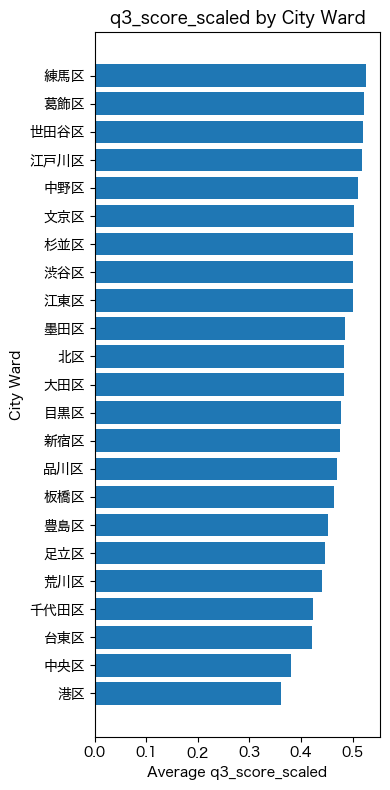
\includegraphics[width=0.45\columnwidth]{plots/tokyo23_q3.png}
    \captionof{figure}{VGA analysis results and q3 impression score distributions across Tokyo's 23 special wards}
    \label{fig:tokyo23_exp}
\end{flushleft}

\section{Conclusion and Future Work}

This research presents a comprehensive framework for analyzing spatial openness in rental housing through automated madori
interpretation, image-based visibility graph analysis, and interior semantic segmentation. Our methodology leverages big data
approaches to quantify subjective spatial qualities using unstructured visual data from rental platforms, demonstrating
scalable processing techniques for large-scale urban analysis. Key findings reveal weak correlations between VGA metrics and
user impression scores, with interior segmentation showing that excessive floor/ceiling visibility negatively impacts quality
perceptions. However, several limitations affect our results: (1) q3 impression scores derive from comparative models with
potential alignment bias and large variance, (2) VGA accuracy depends heavily on semantic segmentation quality, introducing
systematic errors when segmentation fails, and (3) interior segmentation captures only visual element types rather than
aesthetic qualities that significantly influence spatial perception. Future work should address these biases through improved
scoring methodologies, robust segmentation validation, and integration of aesthetic analysis models. Despite limitations, this
open-source framework provides practical tools for real estate professionals and urban planners seeking data-driven spatial
quality assessment, with potential expansion beyond Tokyo and incorporation of 3D spatial information for enhanced analysis.

\section{References}

[References would be listed here.]

\end{multicols}

\newpage

\begin{multicols}{2}
\fontsize{11}{13}\selectfont

% Additional content for page 3 would continue here
% This could include detailed methodology descriptions,
% additional results, or extended discussion sections

\end{multicols}

\newpage

\begin{multicols}{2}
\fontsize{11}{13}\selectfont

% Final page content would be placed here
% This might include appendices, additional references,
% or supplementary analysis results

\end{multicols}

\end{document}